% This program can be redistributed and/or modified under the terms
% of the GNU Public License, version 3.
%
% Seth Brown, Ph.D.
% sethbrown@drbunsen.org
%
% Compiled with XeLaTeX
% Dependencies:
%   Fontin Sans font (http://www.exljbris.com/fontinsans.html)
%
\documentclass{beamer}

\usepackage{graphicx} % graphics
\usepackage{epsfig} % eps graphics
\usepackage{hyperref} % urls
\usepackage{booktabs, caption} % table styling
\usepackage{subfig}
\usepackage{colortbl}
\usepackage[square,authoryear]{natbib}
\usepackage{pgfpages}
%\setbeameroption{show notes on second screen=left}
\definecolor{myblue}{HTML}{D4DEFF}
\definecolor{redcell}{HTML}{FFE8E8}
\definecolor{greencell}{HTML}{E8FFEB}
\definecolor{yellowcell}{HTML}{FFFDE8}
\newcommand{\vomega}{\vec{\omega}}
\newcommand{\x}{\mathbf{x}}
\newcommand{\cs}{C_{\phi}(\eta)}
\newcommand{\csinv}{C_{\phi}(1/\eta)}
\newcommand{\ce}{C_{\mathbf{E}}(\eta)}
\newcommand{\gl}[1]{\texttt{\nolinkurl{#1}}}
\newcommand\mycolor[1]{
\ifnum#1>100 \cellcolor{redcell}#1%
\else
\ifnum#1>60 \cellcolor{yellowcell}#1%
\else
\cellcolor{greencell}#1%
\fi
\fi
}% suppress navigation bar
\beamertemplatenavigationsymbolsempty

\mode<presentation>
{
  \usetheme{bunsen}
  \setbeamercovered{transparent}
  \setbeamertemplate{items}[circle]
}

% set fonts
\usepackage{fontspec}
\setsansfont{Fontin Sans Regular}
\setbeamerfont{frametitle}{size=\LARGE,series=\bfseries}

% color definitions
\usepackage{color}
\definecolor{uipoppy}{RGB}{153, 0, 0}
\definecolor{uipaleblue}{RGB}{153,153,153}
\definecolor{uiblack}{RGB}{0, 0, 0}

% caption styling
\DeclareCaptionFont{uiblack}{\color{uiblack}}
\DeclareCaptionFont{uipoppy}{\color{uipoppy}}
\captionsetup{labelfont={uipoppy},textfont=uiblack}

% see the macros.tex file for definitions
\include{macros}

% title slide definition
\title[Real-time Rendering of Translucent Materials]{Real-time Rendering of Translucent Materials with Directional Subsurface Scattering}
\author{Alessandro Dal Corso}
\institute[DTU Compute]
{
DTU Compute \\
}

\date{7${}^{th}$ November 2014}

%--------------------------------------------------------------------
%                           Introduction
%--------------------------------------------------------------------

\begin{document}

\section{Introduction}
\setbeamertemplate{background}
{\includegraphics[width=\paperwidth,height=\paperheight]{frontpage_bg}}
\setbeamertemplate{footline}[default]

\begin{frame}
\vspace{1cm}
\begin{columns}
\column{2.75in}
  \titlepage
  \vspace{10cm}
\column{2.0in}
\end{columns}
\note{
\begin{itemize}
\item Alessandro, Msc in DME
\item Thesis title: RTR Translucent Materials with Dir SS
\item DTU Compute
\item Supervisor
\end{itemize}
}
\end{frame}

%-------------------------------------------------------------------
%                          Section 1
%-------------------------------------------------------------------
%
% Set the background for the rest of the slides.
% Insert infoline

\setbeamertemplate{background}
 {\includegraphics[width=\paperwidth,height=\paperheight]{slide_bg}}
\setbeamertemplate{footline}[bunsentheme]

\section{Introduction}

\begin{frame}
    \frametitle{Introduction}
\begin{columns}[t]
    \begin{column}{\paperwidth}
      \centering
		\vspace{0.0cm}
		\includegraphics[width=\paperwidth]{comb}
\end{column}
​\end{columns}
\note{
\begin{itemize}
\item Examples in nature
\item Marble, leaves, wax
\item Very present in nature
\end{itemize}
}
\end{frame}

\begin{frame}
    \frametitle{Problem statement}
		Our goal is to represent SS phenomena in a synthetically generated image:
		\vspace{0.5cm}
		\begin{itemize}
			\item Using a analytical BSSRDF model \citep{IMM2013-06646}  
			\item Visually close as possible to a offline-rendered solution
			\item That does not need uv-mapping (only position data)
			\item In real-time or at least at interactive frame rates using a GPUs
		\end{itemize}
		\note{
\begin{itemize}
\item Approach
\item Proposal: use an analytical model (BSSRDF) - opposed to numerical
\item Close to offline - never implemented
\item Low memory requirements (console) 
\item Real time - 100 ms - GPUs
\end{itemize}
}
\end{frame}


\section{Theory}

\begin{frame}
    \frametitle{The rendering equation}
			\begin{itemize}
				\item We use the \emph{area formulation} of the \emph{rendering equation} \citep{Jensen:2001:PMS:383259.383319}:
				$$L_o(\x_o,\vomega_o) = L_e(\x_o,\vomega_o) + \int_A \int_{2\pi} S(\x_i, \vomega_i, \x_o, \vomega_o) L_i(\x_i,\vomega_i) (\vec{n} \cdot \vomega_i) d\vomega_i d A_i$$
				\item Many BSSRDF functions have been proposed in literature \citep{Jensen:2001:PMS:383259.383319,D'Eon:2011:QMR:1964921.1964951,IMM2013-06646}  
			\end{itemize}
\note{
\begin{itemize}
\item Derivation from the previous
\item Add emission and visibility terms
\item Jensen, d'Eon, Jeppe (describe very briefly)
\end{itemize}
}
\end{frame}

\begin{frame}
    \frametitle{Standard dipole}
			\begin{itemize}
			\vspace{0.5cm}
				\item The first BSSRDF model to be proposed for subsurface scattering (depends only on $r$) 
				\item It models the interaction as two small light point sources, a \textcolor{green}{virtual} and a \textcolor{blue}{real} source \\
				\centering
				\vspace{0.2cm}
				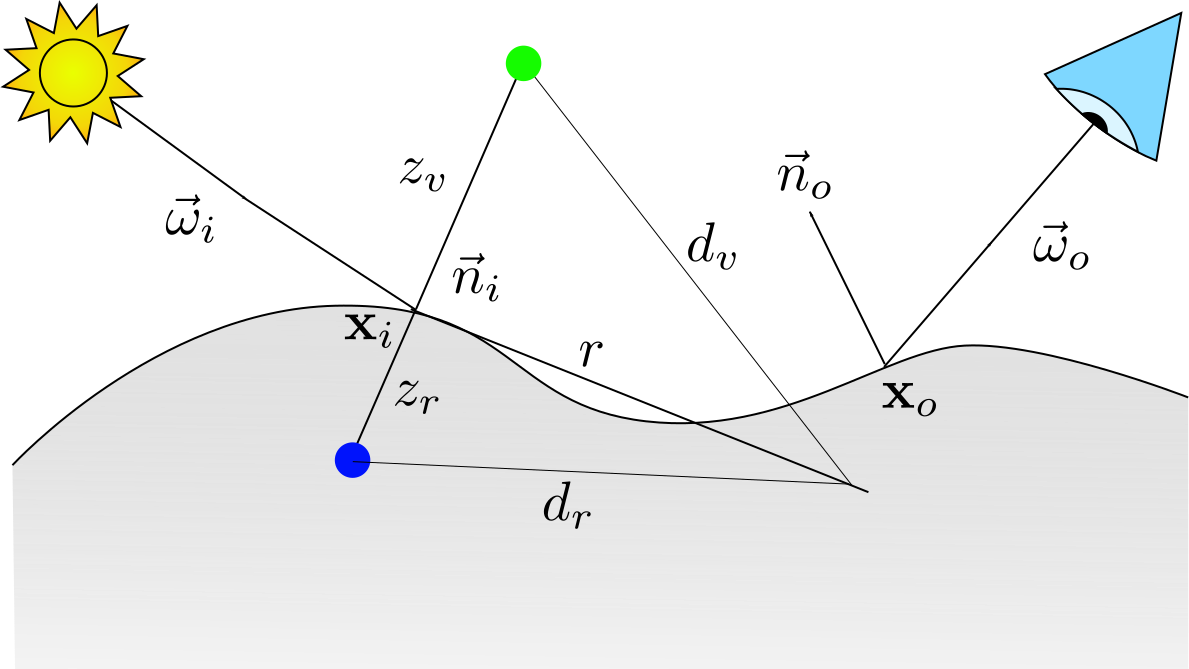
\includegraphics[width=0.55\textwidth]{jensen}
			\end{itemize}
	$$
S_d(\x_i,\vomega_i,\x_i,\vomega_o) = \frac{\alpha'}{4 \pi^2} \left[\frac{z_r (1 + \sigma_{tr} d_r) \; e^{-\sigma_{tr} d_r}}{d_r^3} + \frac{z_v (1 + \sigma_{tr} d_v) \; e^{-\sigma_{tr} d_v}}{d_v^3} \right]
$$			
\note{
\begin{itemize}
\item Boundary conditions (semi infinite medium)
\item z = 2AD (mismatching indices of refraction)
\item we can extend it to arbitrary geometry
\item Solution in the form of a dipole
\item Formula
\end{itemize}
}
\end{frame}

\begin{frame}
    \frametitle{Directional dipole}
		\vspace{0.3cm}
			\begin{itemize}
				\item \citep{IMM2013-06646} defined a new BSSRDF function that keeps the directionality of the incoming light into account \\		
				\item Depends on the direction of the incoming light $\vomega_i$, the two points $\x_o$ and $\x_i$ and the two normals
			\end{itemize}
				\centering
				\vspace{0.2cm}
				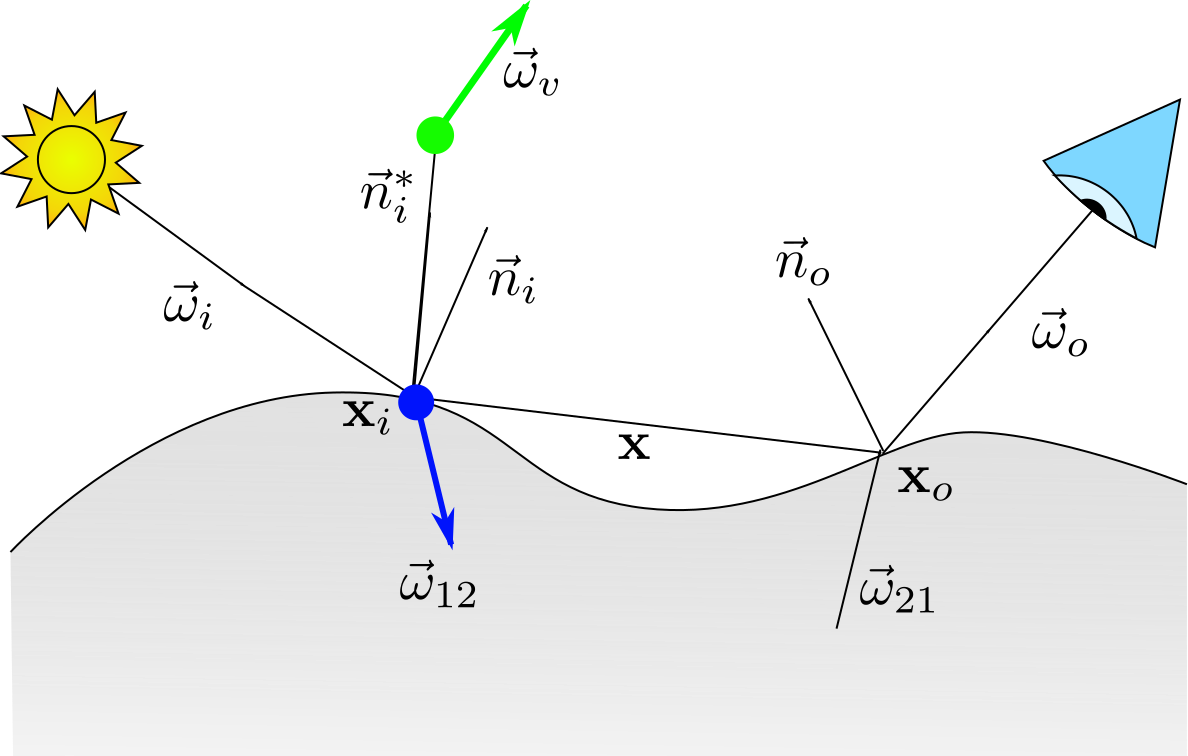
\includegraphics[width=0.55\textwidth]{jeppe}
			$$
			S_d(\x_i, \vomega_i, \x_o) = S'_d(\x_o - \x_i, \vomega_{12}, d_r) - S'_d(\x_o - \x_v, \vomega_{v}, d_v)
			$$
			\note{
\begin{itemize}
\item Extra corrections and boundary conditions
\item Modified tangent plane (show on picture normals)
\item Distance to the real source (changed to avoid singularity - only on real)
\item Formula
\end{itemize}
}

\end{frame}

\section{Method}
\begin{frame}
    \frametitle{Method}
			\begin{itemize}
			\vspace{0.2cm}
			\item Scattering effects have a limited range, that depends on the scattering properties of the material (especially on $1/\sigma_{tr}$)
			\item We can then consider contributions from a disk on the surface
			\item The disk has a center point $\x_d$ and a direction $\vomega_d$
			\end{itemize}
			\centering
			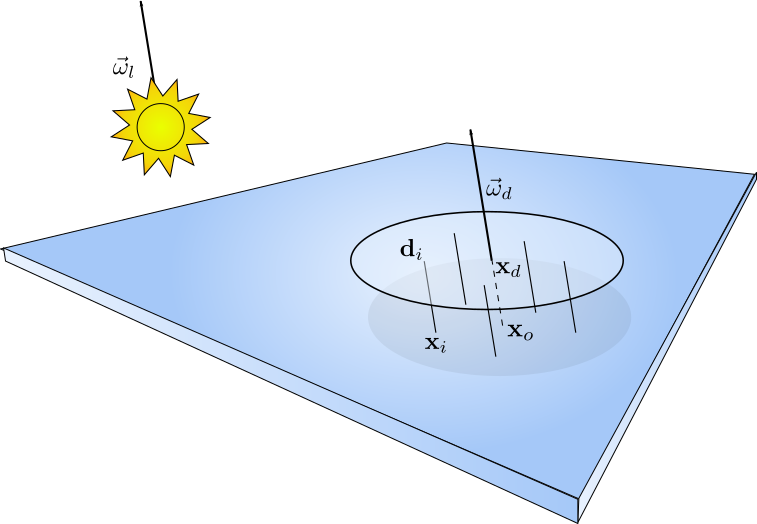
\includegraphics[width=0.55\textwidth]{disk_setup.pdf} 
\note{
\begin{itemize}
\item Rationale behind our approach
\item Limited range - effective transport coefficient
\item We consider only point on a projected disk on a surface
\item Show on image
\item disk has xd and omegad
\end{itemize}
}

\end{frame}

\begin{frame}
    \frametitle{Method}
			\begin{itemize}
			\item We place the disk oriented towards the light ($\vomega_d = \vomega_l$) and close enough to the light in order to cover the surface
			\end{itemize}
			\vspace{0.2cm}
			\begin{columns}
    \begin{column}{0.5\textwidth}
      \centering
		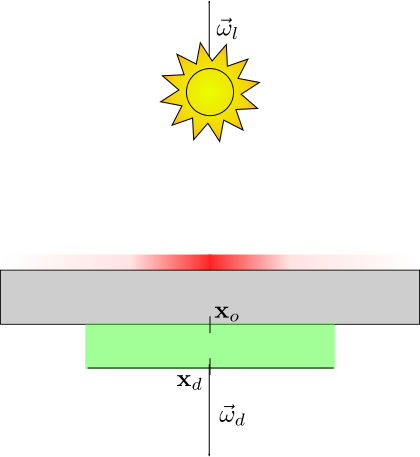
\includegraphics[width=0.8\textwidth]{distribution_wrong_1}
		\\\textit{Naïve disk placement}
				\end{column}
    \begin{column}{0.5\textwidth}
      \centering
		\includegraphics[width=0.8\textwidth]{distribution_wrong_2}
		\\\textit{Our disk placement}
    \end{column}
​  \end{columns}
\note{
\begin{itemize}
\item Describe optimal placement on slab
\item Naive: xo no
\item Our:   x weird, wl
\end{itemize}
}
\end{frame}

\begin{frame}
    \frametitle{Method}
			\begin{itemize}
			\item Given these assumptions on the disk, we discretize the rendering equation (using an uniform sampling):
				$$L_o(\x_o,\vomega_o) = L_e(\x_o,\vomega_o) + \int_A \int_{2\pi} S(\x_i, \vomega_i, \x_o, \vomega_o) L_i(\x_i,\vomega_i) (\vec{n} \cdot \vomega_i) d\vomega_i d A_i$$
				$$
				L_o(\x_o,\vomega_o) = L_d \frac{A_c}{N} \sum_{i = 1}^N S(\x_i, \vomega_d, \x_o, \vomega_o) (\vomega_d \cdot \vec{n}_i)
				$$
   		\item A uniform sampling is not enough, so we need to employ a particular sampling scheme 		
			\end{itemize}

\note{
\begin{itemize}
\item We discretize the rendering eq - only a number of samples N.
\item Sum BSSRDF over points (radiance)
\item Exponential term and images
\end{itemize}
}
\end{frame}

\section{Implementation}
\begin{frame}
    \frametitle{Implementation (step 1)}
			\begin{itemize}
			\item We render the scene from the light point of view (as in \emph{shadow mapping})
			\item We store positions and normals in a texture, the \emph{light map}
			\item We get the closest points to light
			\end{itemize}
			\centering
			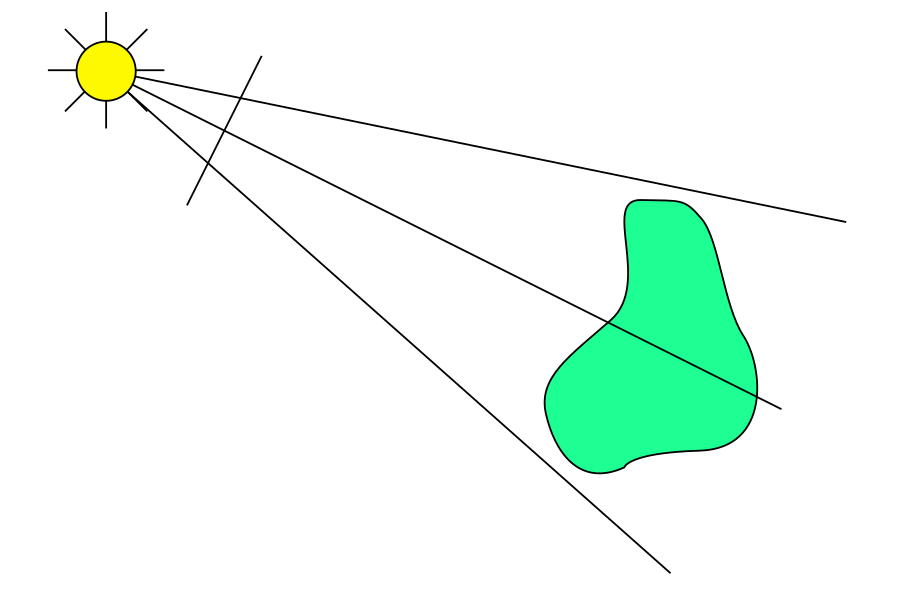
\includegraphics[width=0.5\textwidth]{step1.jpg} 
			\note{
\begin{itemize}
\item Implementation how?
\item Little details - three steps
\item Render to light map
\item Show on image
\item closest point to the light
\end{itemize}
}
\end{frame}

\begin{frame}
    \frametitle{Implementation (step 2)}
			\begin{itemize}
			\item We render the object from a certain number of directions in the \emph{radiance map}
			\item The directions are chosen randomly 
			\item For each pixel we sample the points from the light map and sum up the BSSRDF contribution
			\item The result is accumulated over multiple frames to reduce noise
			\end{itemize}
			\centering
			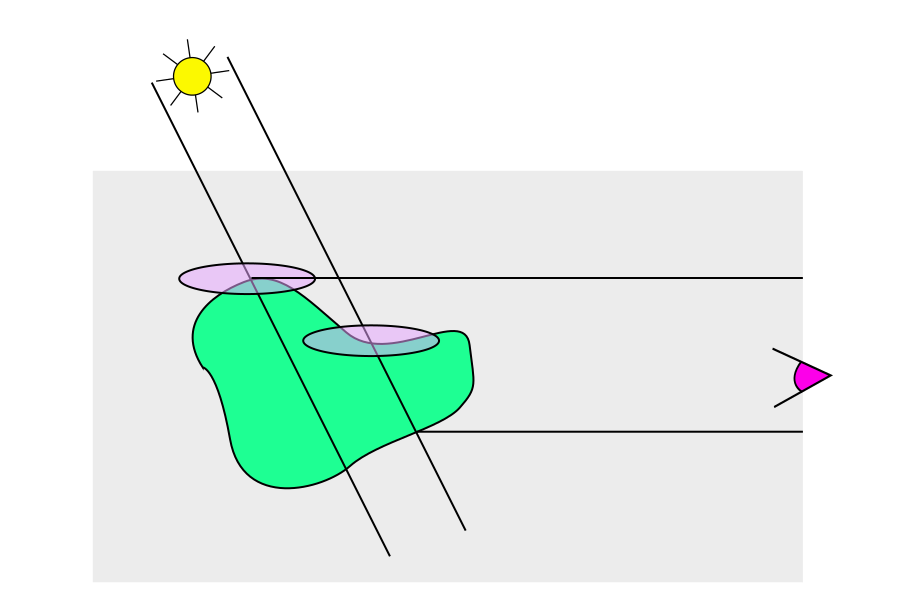
\includegraphics[width=0.35\textwidth]{step2.jpg} 
		\note{
\begin{itemize}
\item Render the object from multiple directions
\item directions random or placed, research on that
\item radiance map
\item fragment shader - sample light maps and accumulate bssrdf as in method
\item Show on image
\end{itemize}
}
\end{frame}

\begin{frame}
    \frametitle{Implementation (step 3)}
			\begin{itemize}
			\item We finally sample the radiance map to get the single contribution for a point on the surface
			\item The result is averaged over the directions from which the surface point is visible
			\end{itemize}
			\centering
			\vspace{-0.5cm}
			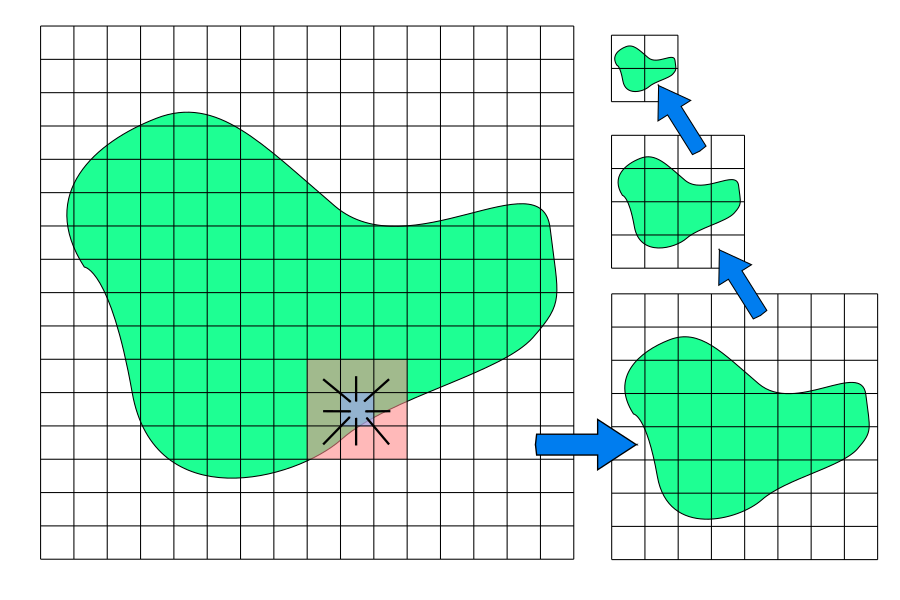
\includegraphics[width=0.4\textwidth]{step3.jpg} 
		\note{
\begin{itemize}
\item Combination - visibility
\item Averaged over directions
\item Depth map
\item Show on image
\end{itemize}
}
\end{frame}

\begin{frame}
    \frametitle{Implementation}
\begin{figure}
\vspace{0.3cm}
\centering
\includegraphics[width=0.55 \textwidth]{bunny}
\vspace{-0.3cm}
\caption{Stanford Bunny, potato material. Note the self shadowing automatically generated by the algorithm.}
\end{figure}
		\note{
\begin{itemize}
\item Result at convergence - bunny potato - real time
\end{itemize}
}
\end{frame}

\begin{frame}
    \frametitle{Advantages}
\begin{itemize}
	\item Accounts for self occlusion
	\item Accounts for occlusion between different objects
	\item Directly coupled with an existing shadow mapping pipeline
	\item Low memory requirements compared to a full voxelization
	\item No UV mapping is necessary
	\item The final step can be adapted to forward and deferred shading pipelines
\end{itemize}
		\note{
\begin{itemize}
\item self shadows
\item occlusion - multiple object
\item coupling shadow mapping comes in!
\item compared to a full voxelization, low memory requirements
\item forward and deferred paths - uncoupling
\end{itemize}
}
\end{frame}


\begin{frame}
    \frametitle{Disadvantages}
\begin{itemize}
	\item Noise, partially overcome by sampling
	\item Cameras that cover the surface need to be placed manually (to avoid tearing)
	\item Inherited problems from shadow mapping (constant shadow bias)
\end{itemize}
	\centering
	\includegraphics[width=0.3 \textwidth]{tearing}
		\note{
\begin{itemize}
\item Noise (see later in videos) - need blurring
\item Tearing
\item Constant shadow bias
\end{itemize}
}
\end{frame}

\begin{frame}
    \frametitle{Results (quality)}
				\begin{figure}
\centering
\subfloat[{1 frame (5 samples)}]{
  \includegraphics[width=0.45 \textwidth]{res_1frame}
}
\subfloat[ ca. 100 frames]{
  \includegraphics[width=0.45 \textwidth]{res_conv}
} 
\vspace{-0.2cm}
\caption{Result comparison for the Stanford Bunny model at different times. Parameters for potato.}
\end{figure}

\end{frame}

\begin{frame}
    \frametitle{Extensions}
\begin{itemize}
\vspace{0.4cm}
	\item \texttt{Multiple lights} \\ We sum the contribution of multiple lights in the shader
	\item \texttt{Point lights} \\ We scale the incoming intensity by a inverse square distance term	
\end{itemize}
      \centering
		\includegraphics[width=0.4\textwidth]{point}
\end{frame}

\begin{frame}
    \frametitle{Environment lighting}
\begin{itemize}
	\item We simulate it using 16 directional lights 
	\item We choose "random" points on a environment map 
	\item The distribution chosen accounts to make the points fall in areas with high luminosity
\end{itemize}
      \centering
		\includegraphics[width=0.4\textwidth]{skymap}
				\note{
\begin{itemize}
\item Environment lighting
\item 16 directional lights from a environment map
\item Chosen on a distribution - more probable to have points on areas with higher luminosity  
\item show image
\end{itemize}
}
\end{frame}

\section{Results}

\begin{frame}
    \frametitle{Results (quality)}
				\begin{figure}
\centering
\subfloat[Our method]{
  \includegraphics[width=0.45 \textwidth]{bunnyour}
}
\subfloat[Reference ]{
  \includegraphics[width=0.45 \textwidth]{bunnyref}
} 
\vspace{-0.2cm}
\caption{Result comparison for the Stanford Bunny model. Parameters for marble.}
\end{figure}
\note{
\begin{itemize}
\item Dragon - around 50000 vertices (simplified)
\item Missing highlights in ketchup
\item Improvements in the time of five orders of magnitude
\item 16 millions samples prior to rejection
\end{itemize}
}
\end{frame}


\begin{frame}
    \frametitle{Results (quality)}
				\begin{figure}
\centering
\subfloat[Our method]{
  \includegraphics[width=0.45 \textwidth]{d50}
}
\subfloat[$\ $Reference (6 hours, 16 millions samples)]{
  \includegraphics[width=0.45 \textwidth]{d}
} 
\vspace{-0.2cm}
\caption{Result comparison for the Stanford Dragon model. Parameters for ketchup.}
\end{figure}
\note{
\begin{itemize}
\item Dragon - around 50000 vertices (simplified)
\item Missing highlights in ketchup
\item Improvements in the time of five orders of magnitude
\item 16 millions samples prior to rejection
\end{itemize}
}
\end{frame}

\begin{frame}
    \frametitle{Results (quality)}
				\begin{figure}
\centering
\subfloat[{Our result}]{
  \includegraphics[width=0.45 \textwidth]{b100}
}
\subfloat[$\ $Reference (30 minutes, $10^6$ samples)]{
\makebox[.5\textwidth]{  \includegraphics[width=0.45 \textwidth]{bref}
}
} 
\vspace{-0.1cm}
\caption{Result comparison for the Happy Buddha model. Parameters for potato.}
\note{
\begin{itemize}
\item Buddha - big model (millions of vertices)
\item 300 ms
\item potato
\item Lose details
\item Little greenish tone
\item General appearance is captured - more work should be done in order to get the highlights
\end{itemize}
}
\end{figure}

\end{frame}

\begin{frame}
    \frametitle{Results (performance)}
\renewcommand{\arraystretch}{1.8}
\begin{table}[!ht]
\centering
\begin{tabular}{p{3cm}l|l|l|l|l|}
\cline{3-6}
                             &      & \multicolumn{4}{c|}{Number of samples ($N$)}                                          \\ \cline{3-6} 
Model                        & \#$\Delta$& \multicolumn{1}{c|}{1} & \multicolumn{1}{c|}{10} & \multicolumn{1}{c|}{50} & \multicolumn{1}{c|}{100} \\ \hline
\multicolumn{1}{|l|}{Bunny}  & $10^4$ & \mycolor{2}.1                  & \mycolor{5}.3                 & \mycolor{19}.8                  & \mycolor{38}.2                 \\ \hline
\multicolumn{1}{|l|}{Dragon} & $10^5$ & \mycolor{12}.5                 & \mycolor{35}.2                  & \mycolor{140}.6                & \mycolor{275}.3                \\ \hline
\multicolumn{1}{|l|}{Buddha} & $10^6$ & \mycolor{96}.7                 & \mycolor{97}.7                  & \mycolor{128}.0                & \mycolor{216}.0                 \\ \hline
\end{tabular}
\caption{Timings in milliseconds of our method for different models and number of samples $N$ (potato material properties). One directional light, 16 directions for rendering and reconstructing.}
\end{table}
\note{
\begin{itemize}
\item color code
\item Performance increase with N
\item 16 directions is conservative (random)
\item explain why buddha rises less than dragon (area occupation)
\item at low N rasterization wins
\end{itemize}
}
\end{frame}

\section{Current work}
\begin{frame}
    \frametitle{Conclusions}
What I did so far:
\begin{itemize}
\item Improved sampling (various corrections)
\item Moved to a GPU random number generation (vs. texture-based)
\item Introduced spectrally based computation
\item Finite difference compensation term for different sampling terms
\end{itemize}
What are the next steps:
\begin{itemize}
\item Remove undesired color shifts
\item Implement fast denoising for the final of the algorithm
\item Comparison in performance with Optix ray-traced solution (special course)
\end{itemize}
\note{
\begin{itemize}
\item Fast rendering
\item Results comparables
\item Five orders
\item Flexible - in engines
\end{itemize}
}

\end{frame}

\begin{frame}
    \frametitle{Conclusions}
\centering
\includegraphics[width=0.4\textwidth]{front} \\
\huge Thank you!
\end{frame}

\section{References}

\begin{frame}
    \frametitle{References}
\bibliographystyle{alexnat}                           %Use alpha codes for references
\bibliography{thesis} 
\end{frame}

\begin{frame}
    \frametitle{Notes on sampling}
\centering
\includegraphics[width=0.4\textwidth]{front} \\
\huge Thank you!
\end{frame}


\end{document}
